\chapter{Analyse et spécification des besoins}

L'analyse transforme la problématique en fonctions mesurables et en contraintes de qualité applicables aux trois profils de la plateforme.


\section{Identification des acteurs}

{\small\singlespacing\arrayrulecolor{tableline}
\begin{longtable}{|>{\raggedright\arraybackslash}p{\dimexpr 0.350\textwidth-2\tabcolsep-2\arrayrulewidth\relax}|>{\raggedright\arraybackslash}p{\dimexpr 0.650\textwidth-2\tabcolsep-2\arrayrulewidth\relax}|}
\hline
\rowcolor{tablehead} \color{white}\bfseries Acteur & \color{white}\bfseries Responsabilités et objectifs \\ \hline
\endfirsthead
\rowcolor{tablehead} \color{white}\bfseries Acteur & \color{white}\bfseries Responsabilités et objectifs \\ \hline
\endhead
\hline\endfoot
Visiteur & Consulter le catalogue public, filtrer et ouvrir une annonce sans accéder aux coordonnées privées. \\ \hline
\rowcolor{tablerow} Acheteur & Gérer son profil et ses véhicules, sauvegarder, contacter, échanger, signaler et évaluer un vendeur éligible. \\ \hline
Vendeur & Gérer ses annonces, images, compatibilités et statuts, répondre aux conversations et suivre sa réputation. \\ \hline
\rowcolor{tablerow} Administrateur & Valider les vendeurs, modérer annonces et signalements, suspendre des comptes et consulter l'audit. \\ \hline
\end{longtable}
}


\section{Besoins fonctionnels}

\begin{itemize}
\item inscription par courriel et mot de passe, connexion OAuth facultative, récupération par courriel ou téléphone ;

\item édition d'un profil complet avec coordonnées, localisation, activité, biographie et site web ;

\item demande de passage vendeur placée en attente jusqu'à décision de l'administrateur ;

\item cycle de vie d'une annonce : saisie et aperçu avant publication, modification, activation, désactivation, vente et suppression ; les états persistés sont ACTIVE, INACTIVE et SOLD ;

\item ajout, compression, prévisualisation, ordre par glisser-déposer, choix de l'image principale et suppression ;

\item recherche par catégorie, marque, modèle, année, carburant, moteur, position, prix, livraison, état et tri ;

\item recherche en langage naturel avec contraintes comprises et raisons de correspondance ;

\item contact protégé par téléphone, WhatsApp, courriel et messagerie interne avec pièces jointes ;

\item avis de 1 à 5 étoiles, commentaire facultatif, réputation agrégée et signalement vendeur ;

\item tableau de bord administrateur, files de traitement et journal d'audit ;

\item recommandations personnalisées, paramètres de confidentialité et effacement de l'historique de recommandation.
\end{itemize}

\section{Besoins non fonctionnels}

{\small\singlespacing\arrayrulecolor{tableline}
\begin{longtable}{|>{\raggedright\arraybackslash}p{\dimexpr 0.350\textwidth-2\tabcolsep-2\arrayrulewidth\relax}|>{\raggedright\arraybackslash}p{\dimexpr 0.650\textwidth-2\tabcolsep-2\arrayrulewidth\relax}|}
\hline
\rowcolor{tablehead} \color{white}\bfseries Axe & \color{white}\bfseries Exigence retenue \\ \hline
\endfirsthead
\rowcolor{tablehead} \color{white}\bfseries Axe & \color{white}\bfseries Exigence retenue \\ \hline
\endhead
\hline\endfoot
Sécurité & JWT signé, mots de passe hachés, RBAC, secrets hors dépôt, validation de fichiers et limitation de débit. \\ \hline
\rowcolor{tablerow} Fiabilité & MySQL reste la source de vérité ; un index obsolète ne doit pas exposer une annonce devenue inactive. \\ \hline
Explicabilité & Toute recommandation et tout résultat IA affichent des raisons issues de données contrôlées. \\ \hline
\rowcolor{tablerow} Performance & Pagination, cache court, seuil de pertinence, concurrence bornée et images compressées. \\ \hline
Ergonomie & Interface responsive, états de chargement, erreurs lisibles, thème clair/sombre géométriquement stable. \\ \hline
\rowcolor{tablerow} Maintenabilité & Séparation contrôleur/service/dépôt, DTO dédiés, configuration externalisée et tests automatisés. \\ \hline
Confidentialité & Coordonnées réservées aux acheteurs connectés ; historique IA minimal et effaçable. \\ \hline
\rowcolor{tablerow} Portabilité & Services exécutables localement sur Windows pour la démonstration académique. \\ \hline
\end{longtable}
}


\section{Règles métier centrales}

1. Une annonce publique doit être active, appartenir à un vendeur non suspendu et contenir des données valides.


2. Une annonce marquée vendue disparaît immédiatement des listes, recherches et recommandations publiques.


3. Les coordonnées du vendeur ne sont révélées qu'à un acheteur authentifié.


4. Le passage au rôle vendeur exige une demande et une décision explicite de l'administrateur.


5. Une compatibilité multi-véhicule est évaluée ligne par ligne ; le système ne combine jamais la marque d'une ligne avec le carburant d'une autre.


6. La sortie du modèle de langage est une proposition de contraintes, jamais une preuve de compatibilité.


7. Les messages sont réservés aux participants autorisés ; les avis publiés sont consultables sur le profil vendeur.


8. Chaque décision administrative sensible produit une entrée d'audit.


\section{Matrice de traçabilité}

{\small\singlespacing\arrayrulecolor{tableline}
\begin{longtable}{|>{\raggedright\arraybackslash}p{\dimexpr 0.240\textwidth-2\tabcolsep-2\arrayrulewidth\relax}|>{\raggedright\arraybackslash}p{\dimexpr 0.320\textwidth-2\tabcolsep-2\arrayrulewidth\relax}|>{\raggedright\arraybackslash}p{\dimexpr 0.440\textwidth-2\tabcolsep-2\arrayrulewidth\relax}|}
\hline
\rowcolor{tablehead} \color{white}\bfseries Besoin & \color{white}\bfseries Composant responsable & \color{white}\bfseries Validation \\ \hline
\endfirsthead
\rowcolor{tablehead} \color{white}\bfseries Besoin & \color{white}\bfseries Composant responsable & \color{white}\bfseries Validation \\ \hline
\endhead
\hline\endfoot
Authentifier & Spring Security, JWT, OAuth2 & Tests de rôles et parcours navigateur \\ \hline
\rowcolor{tablerow} Publier une annonce & PartService, Angular Seller Studio & CRUD, DTO, upload et statuts \\ \hline
Vérifier la compatibilité & FastAPI + règles déterministes Spring & Jeux multilingues et contradictions \\ \hline
\rowcolor{tablerow} Communiquer & MessagingService, WebSocket & Conversation privée et pièces jointes \\ \hline
Modérer & AdminService, audit & Files de signalement et suspension \\ \hline
\rowcolor{tablerow} Recommander & RecommendationService, agents en lecture & Scénarios de préférences, exclusion et diversité \\ \hline
\end{longtable}
}


\section{Diagrammes de cas d'utilisation}

La frontière E-biessa comprend Angular, Spring Boot et le service FastAPI. Les acteurs humains déclenchent les opérations autorisées ; les services internes ne sont donc pas des acteurs externes dans ces diagrammes. Les vues regroupent les opérations proches pour conserver une lecture globale. Une association indique une interaction, pas une relation de succession.


\clearpage

\subsection{Parcours de consultation et d'achat}

\begin{figure}[H]
\centering
\begin{adjustbox}{max width=\textwidth,max height=.64\textheight}
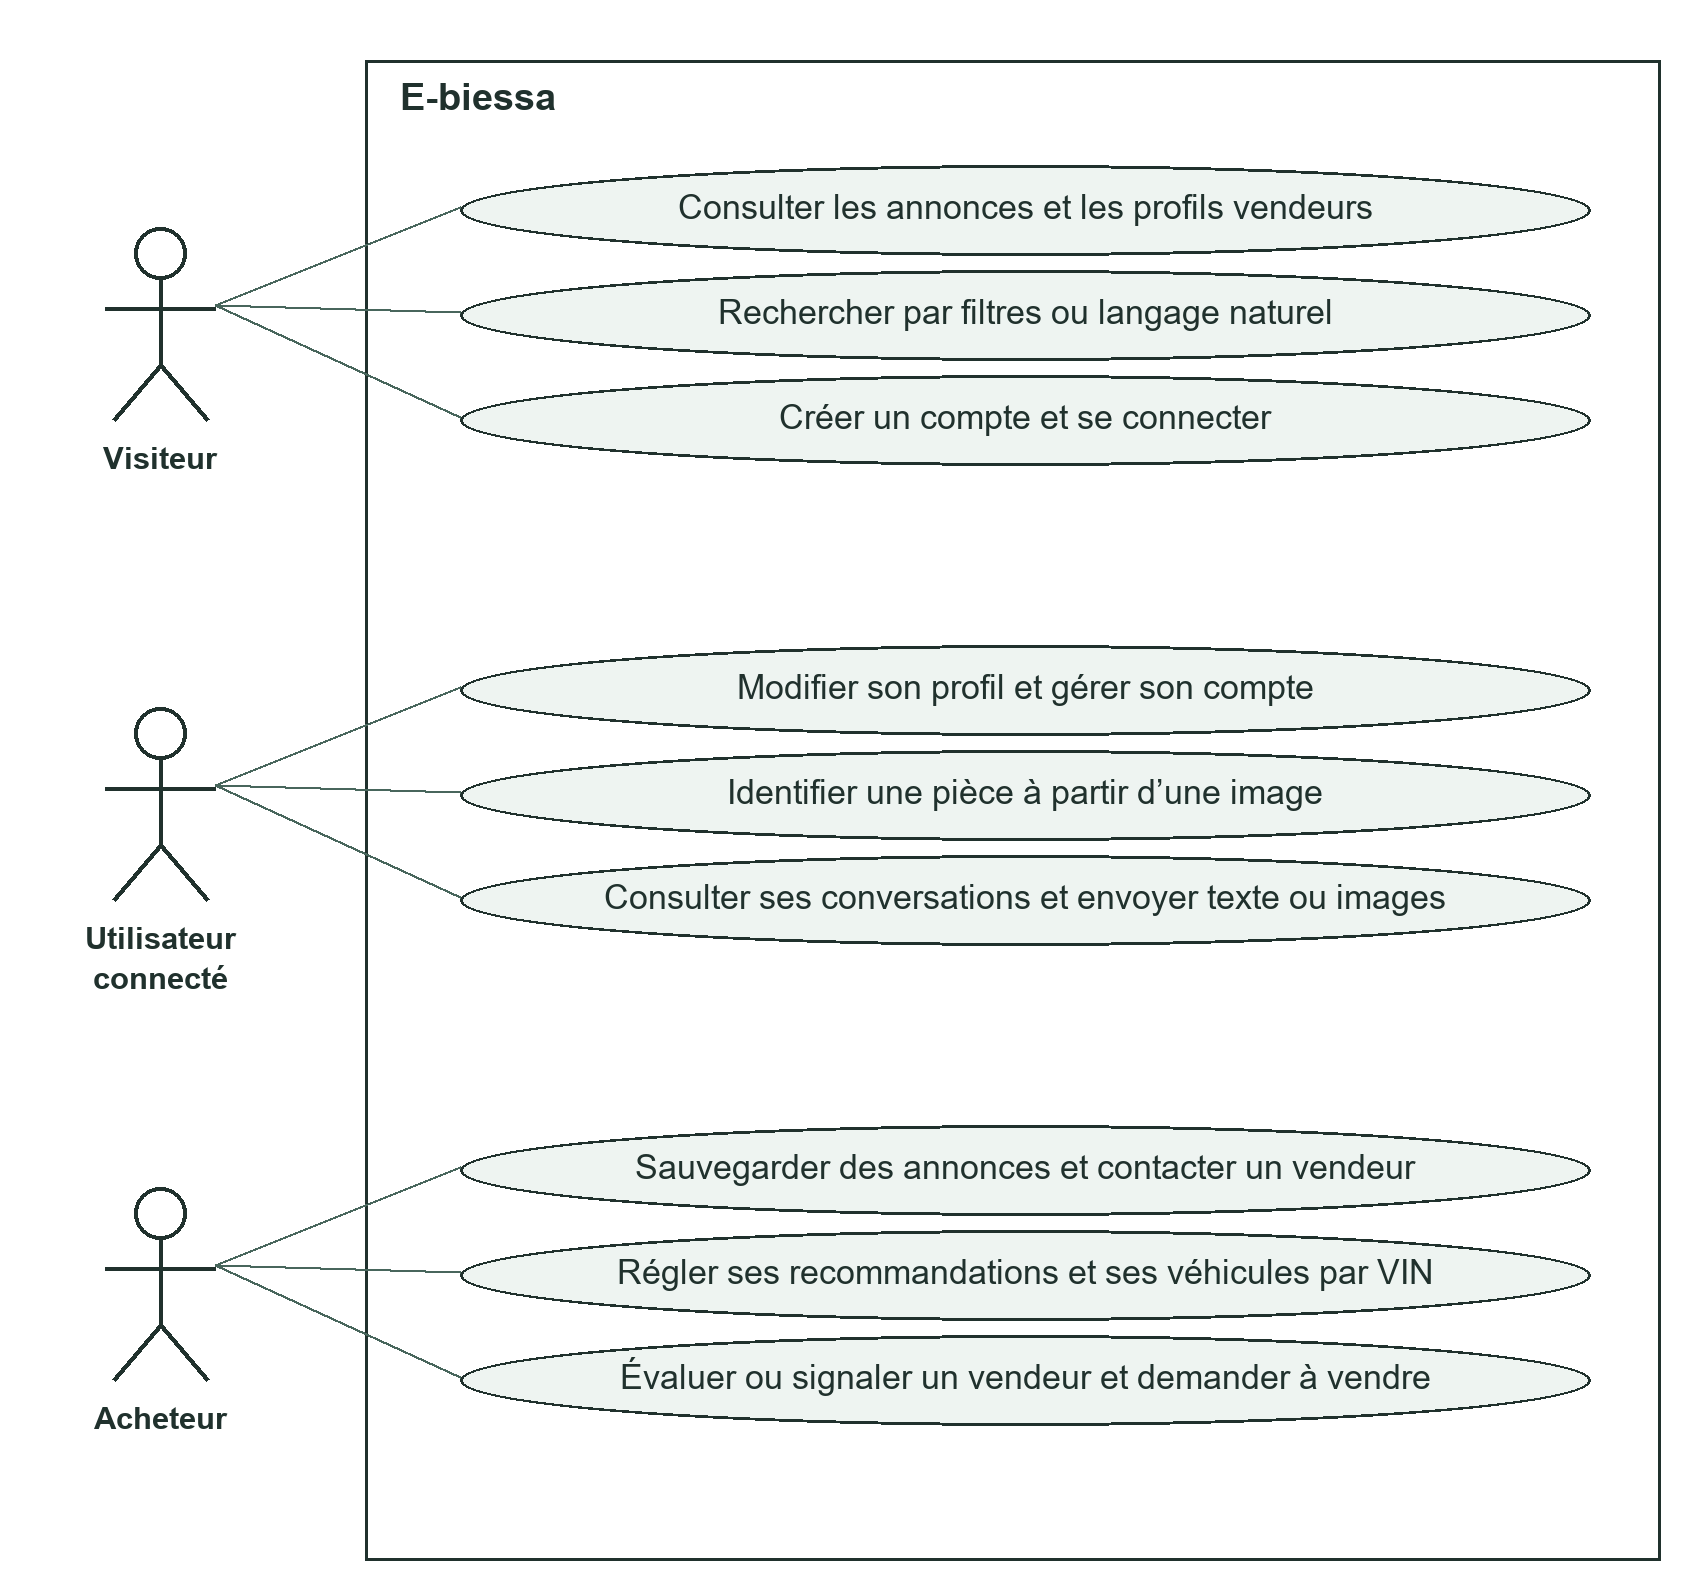
\includegraphics{images/figure-01.png}
\end{adjustbox}

\caption{Cas d'utilisation de consultation et d'achat}
\label{fig:report-1}
\end{figure}

Les fonctions d'utilisateur connecté sont communes aux rôles authentifiés. Les coordonnées, les avis et les recommandations personnalisées restent soumis aux contrôles du rôle acheteur. L'expression « achat » désigne ici la recherche et la mise en relation, sans paiement intégré.


\clearpage

\subsection{Publication et administration}

\begin{figure}[H]
\centering
\begin{adjustbox}{max width=\textwidth,max height=.64\textheight}
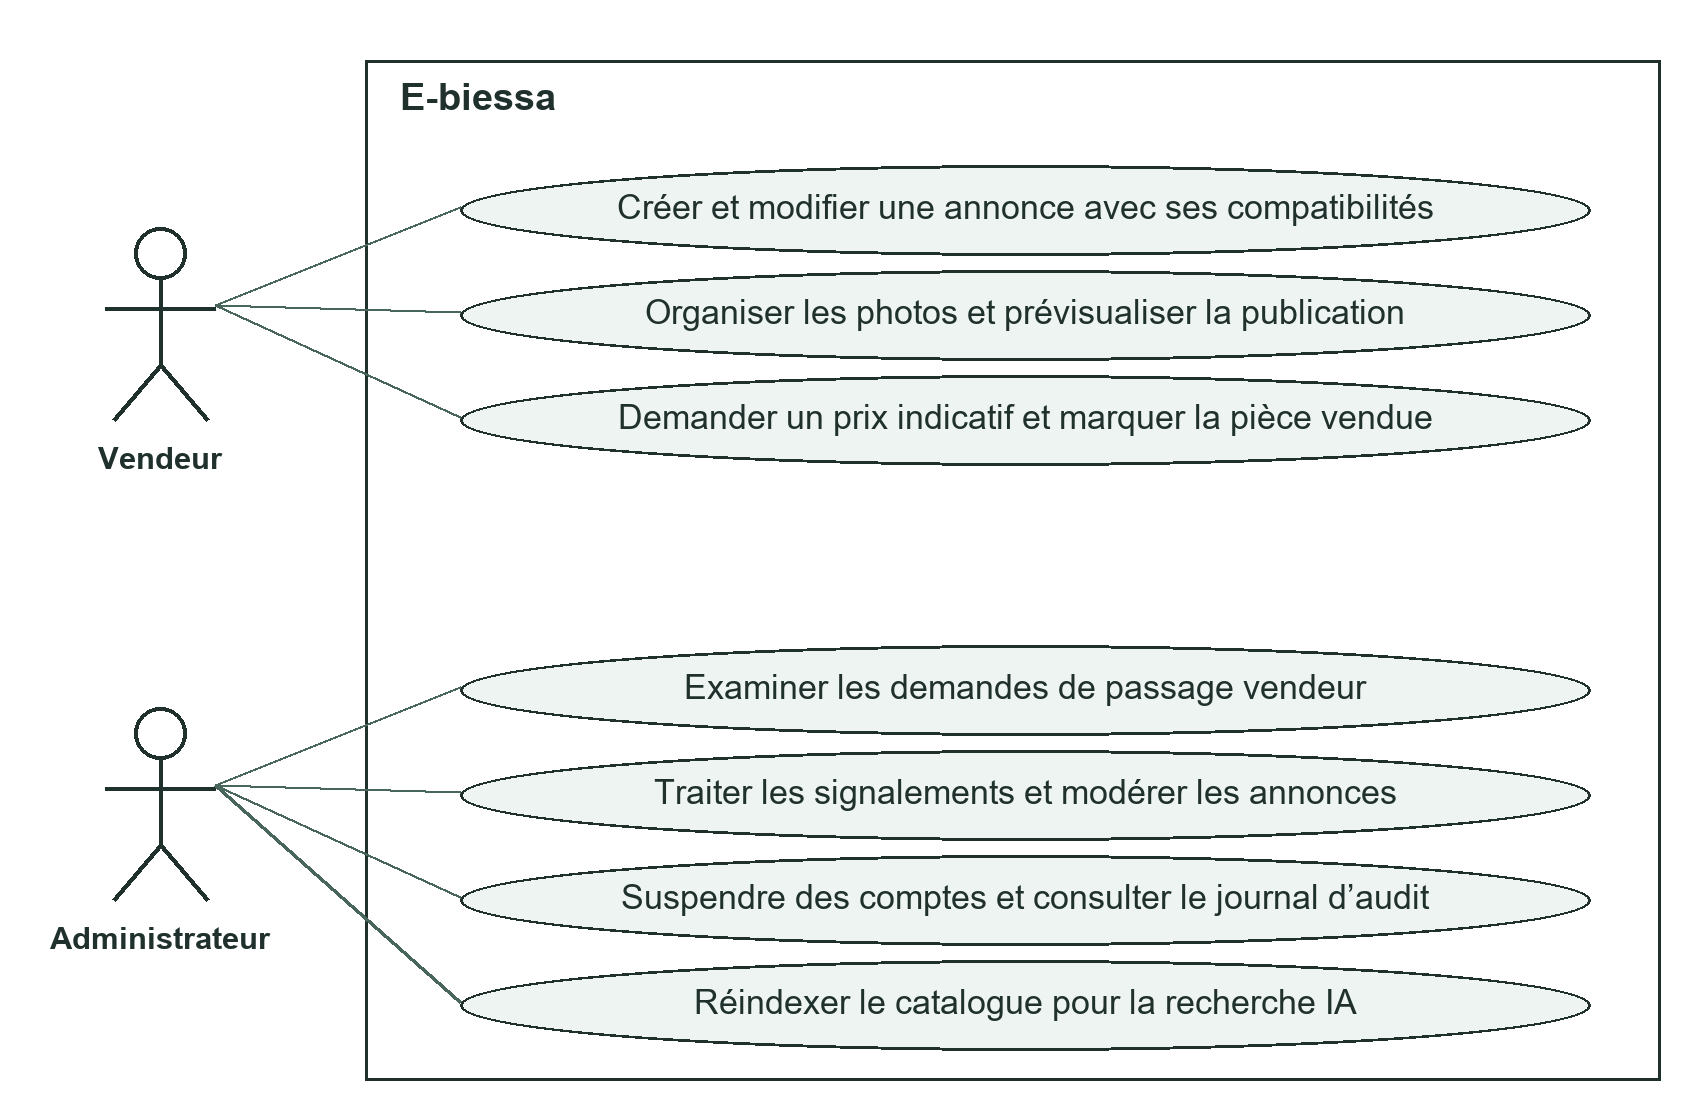
\includegraphics{images/figure-02.png}
\end{adjustbox}

\caption{Cas d'utilisation de vente et d'administration}
\label{fig:report-2}
\end{figure}

Le vendeur bénéficie des fonctions communes de compte et de messagerie. L'administrateur possède également les droits de gestion des annonces autorisés par le backend. La suspension et la résolution des signalements donnent lieu à des traces d'audit.


\subsection{Services externes et variantes}

{\small\singlespacing\arrayrulecolor{tableline}
\begin{longtable}{|>{\raggedright\arraybackslash}p{\dimexpr 0.350\textwidth-2\tabcolsep-2\arrayrulewidth\relax}|>{\raggedright\arraybackslash}p{\dimexpr 0.650\textwidth-2\tabcolsep-2\arrayrulewidth\relax}|}
\hline
\rowcolor{tablehead} \color{white}\bfseries Service externe & \color{white}\bfseries Interaction avec E-biessa \\ \hline
\endfirsthead
\rowcolor{tablehead} \color{white}\bfseries Service externe & \color{white}\bfseries Interaction avec E-biessa \\ \hline
\endhead
\hline\endfoot
Google, Facebook, Microsoft & Connexion OAuth quand le fournisseur est configuré. \\ \hline
\rowcolor{tablerow} SMTP et Twilio & Acheminement des codes de récupération selon la configuration. \\ \hline
CarQuery et NHTSA vPIC & Catalogue automobile et décodage VIN, avec limites de couverture. \\ \hline
\rowcolor{tablerow} Cloudinary & Stockage optionnel des images à la place du stockage local. \\ \hline
Service vocal du navigateur & Transcription soumise au support et aux permissions du navigateur. \\ \hline
\end{longtable}
}


Pour publier, le vendeur saisit les informations, consulte l'aperçu puis confirme l'envoi ; le serveur valide les champs et la propriété. Pour devenir vendeur, l'acheteur transmet sa demande et reste acheteur pendant l'examen. L'administrateur accepte ou refuse ; le rôle ne change qu'en cas d'acceptation. Pour contacter un vendeur, l'acheteur se connecte, ouvre une annonce active puis utilise les coordonnées autorisées ou crée une conversation.
